\section{Diverse}

%\begin{table}[H]
%\centering
%\begin{tabular}{| l | l | l | l | l |}
%\hline
%\textbf{Nr.} 	& \textbf{Average height error [m]} 	& \textbf{Average cross track error [m]} & \textbf{Lateral control system - Lookahead distance [m]} &  \textbf{Rotation combination - approach path} \\ \hline
%$1$				& $1.5$							& $6.1$	&	$ 50 $ 	& Clockwise/ Counter-clockwise							\\ \hline
%$2$				& $2.6$							& $6.7$	& $ 50 $	& Clockwise/ Counter-clockwise							\\ \hline
%$3$				& $0.9$							& $5.5$	& $ 50 $	& Clockwise/ Counter-clockwise							\\ \hline
%$4$				& $0.1$							& $2.8$	& $ 50 $ 	& Counter-clockwise/ Counter-clockwise							\\ \hline
%$5$				& $1.7$							& $2.0$	& $ 50 $ 	& Counter-clockwise/ Counter-clockwise							\\ \hline
%$6$				& $1.3$							& $6.8$	& $ 50 $ 	& Counter-clockwise/ Counter-clockwise							\\ \hline
%$7$				& $1,8$							& $9.1$	& $ 50 $ 	& Counter-clockwise/ Counter-clockwise							\\ \hline
%$8$				& $1.2$							& $8.2$	& $ 50 $ 	& Counter-clockwise/ Counter-clockwise							\\ \hline
%$9$				& $1.9$							& $5.9$	& $ 50 $ 	& Counter-clockwise/ Counter-clockwise							\\ \hline
%$10$			& $1.5$							& $4.4$	& $ 30 $ 	& Counter-clockwise/ Counter-clockwise							\\ \hline
%$11$			& $1.5$							& $1.4$	& $ 30 $ 	& Counter-clockwise/ Counter-clockwise							\\ \hline
%Average			& $1.5$							& $5.4$								\\ \hline
%Variance		& $0.4$							& $6.2$								\\ \hline
%\end{tabular}
%\caption{Mean height and cross track error from day 1}
%\label{tb:Day1HeightCrossTrack}
%\end{table}


%\begin{table}[H]
%
%\begin{tabular}{| p{0.5cm} | p{1cm} | p{1cm} | p{2cm} | p{3cm} | p{2.8cm} |}
%\hline
%\textbf{Nr.}	& \textbf{Height error - net passing [m]}	& \textbf{Cross track error - net passing [m]}& \textbf{Final approach angle [deg]} & \textbf{Lateral control system - Lookahead distance [m]} &  \textbf{Rotation combination - approach path}\\ \hline
%$1$				& $2.8$		& $2.1$	& $3$ &	$ 50 $ 	& Clockwise/ Counter-clockwise		\\ \hline
%$2$				& $2.7$		& $-4.5$ & $0$ & $ 50 $	& Clockwise/ Counter-clockwise			\\ \hline
%$3$				& $0.9$		& $-1.6$ & $0$ & $ 50 $	& Clockwise/ Counter-clockwise		\\ \hline
%$4$				& $0.0$		& $5.4$	& $0$ & $ 50 $ 	& Counter-clockwise/ Counter-clockwise				\\ \hline
%$5$				& $0.8$		& $5.3$	& $0$ & $ 50 $ & Counter-clockwise/ Counter-clockwise					\\ \hline
%$6$				& $2.1$		& $-1.6$ & $0$ & $ 50 $	& Counter-clockwise/ Counter-clockwise				\\ \hline
%$7$				& $0.7$		& $2.3$ & $0$ &	$ 50 $ & Counter-clockwise/ Counter-clockwise				\\ \hline
%$8$				& $-1.5$	& $-5.4$ & $0$ & $ 50 $	& Counter-clockwise/ Counter-clockwise				\\ \hline
%$9$				& $1.9$		& $0.8$ & $0$ & $ 50 $ & Counter-clockwise/ Counter-clockwise			\\ \hline
%$10$			& $0.3$	& $1.1$ & $0$ &	$ 30 $ & Counter-clockwise/ Counter-clockwise	\\ \hline
%$11$			& $-1.3$	& $0.2$ & $0$ & $ 30 $ & Counter-clockwise/ Counter-clockwise\\ \hline
%\end{tabular}
%\caption{Table containing the result of each landing attempt}
%\label{tb:Day1LandingAttempt}
%\end{table}



\subsubsection{First plan}\label{sss:Day1FirstPlan}
The first test of the autonomous landing system was performed with the landing plan parameter listen in appendix \ref{AP:SpecDay1}, which resulted in the path shown in figure \ref{Fig:NorthEast31mai103029}, where the the start position of the landing plan is marked with a circle, the net position with a cross, the desired path as a whole line and the actual flight path as a stippled line. The desired heigh as well as the actual height is shown in figure \ref{Fig:Height31mai103029}. The rotation direction of the start turning circle was chosen to be opposite to the finish turning circle, which resulted in a straight line path between the two turning circles bringing the \gls{uav} into the cross wind. The effect of flying in the cross wind introduced oscillatory motion in the \gls{uav}, which the lateral control system was unable to compensate for. The effect of the oscillatory motion affected the \gls{uav} when entering the finish turning circle, where the result was the \gls{uav} overshooting the desired path. The consequence of the \gls{uav} overshooting the finish turning circle can in the worst case result in the \gls{uav} to leave the line of sight of the pilot, which is a failure when flying in a LOS operation. The \gls{uav} continues to oscillate when flying along the landing path, however the cross track error was within the acceptance criteria listed in table \ref{tb:NetCriteria} at the time the \gls{uav} passed the virtual net.

The longitudinal control system was able to follow it's desired height reference during the approach path, however the \gls{uav} height starts to diverge from the desired height during the landing path. The divergence corresponds to the overshot in the lateral plan, which could be the reason for the divergence. However the desired height from the longitudinal control system was higher then the net center height at the time the \gls{uav} passed the virtual net. The reason behind this behaviour is due to the reference model in the longitudinal control system attempt to create a smooth glide slope towards the aiming position behind the net, which cause the desired height to lag behind the desired path. This behaviour can be removed by setting the final approach angle to zero, thus ensuring that the straight line through the net center has a constant height value.
\begin{figure}[H]
	\centering
		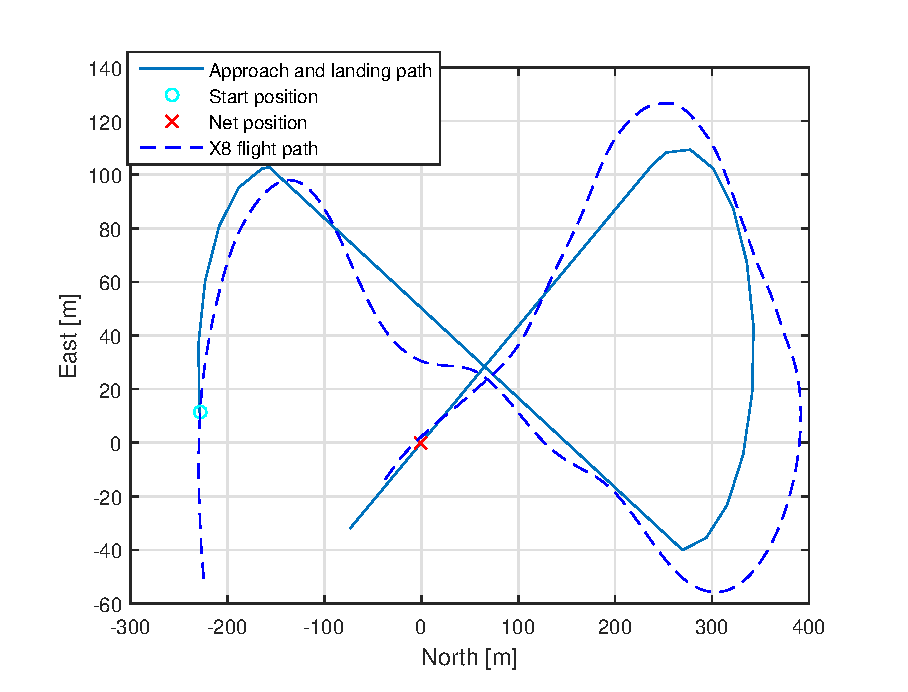
\includegraphics[scale=0.7]{figs/Experiment/NorthEast31mai103029.eps}
		\caption{North-East plot where the start and finish turning circles have opposite turning directions}
		\label{Fig:NorthEast31mai103029}
\end{figure}
\begin{figure}[H]
\centering
		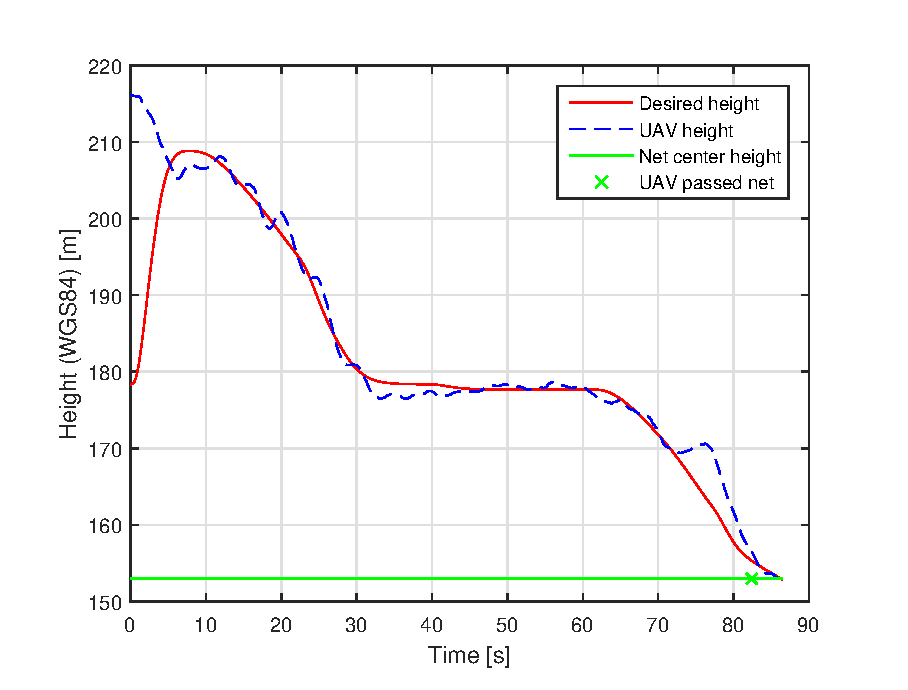
\includegraphics[scale=0.7]{figs/Experiment/Height31mai103029.eps}
		\caption{Height profile of a landing plan with $3 \deg$ net impact angle}
		\label{Fig:Height31mai103029}
\end{figure}

\subsubsection{Path with $\gamma_n = 0$}
A landing plan with the final approach angle ,$\gamma_n = 0$, was created, where the desired and actual height of the \gls{uav} is shown in figure\ref{Fig:Height31mai31mai105034}. The effect of setting the net impact angle to zero gave a better performance from the longitudinal control system, due to the desired height now converging to the net center height. At the time the \gls{uav} passed the virtual net the hight error with respect the height of the net center was within the height error acceptance.
\begin{figure}[H]
\centering
		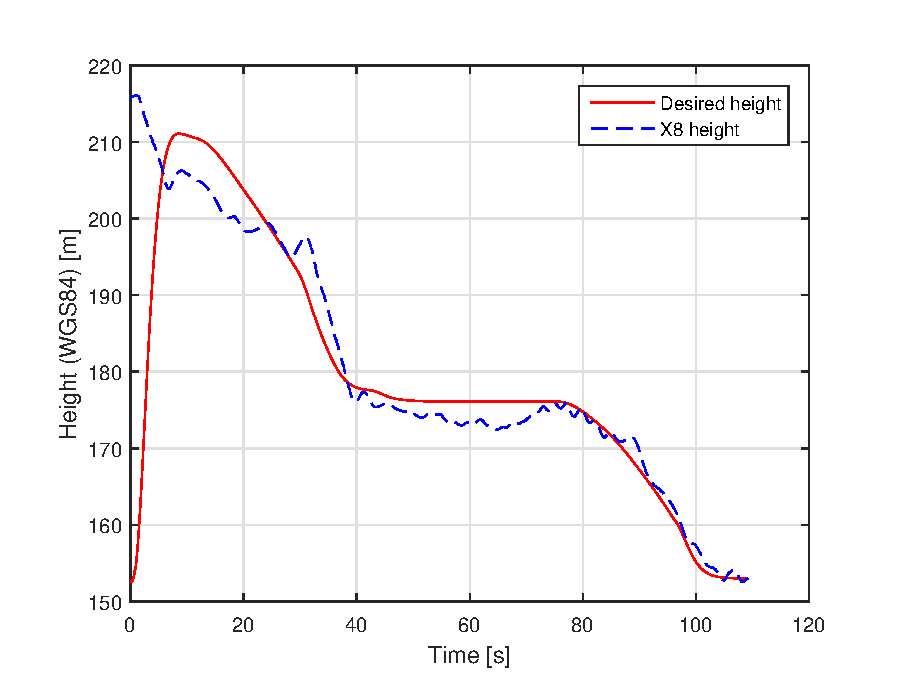
\includegraphics[scale=0.7]{figs/Experiment/Height31mai105034.eps}
		\caption{Height profile of a landing plan with $0 \deg$ net impact angle}
		\label{Fig:Height31mai31mai105034}
\end{figure}

\subsubsection{Path with inverted rotation direction in the start circle}
A landing plan with the rotation direction of the start turning circle inverted with respect to the previous landing plan, as shown in figure \ref{Fig:NorthEast31mai125420}. The result of this alteration was reduced oscillation in the lateral plane for the \gls{uav} when flying along the straight line between the turning circles. The \gls{uav} still experience overshot in the finish turning circle, however the overshooting is reduced due to more stable entry into the finish turning circle.
\begin{figure}[H]
	\centering
	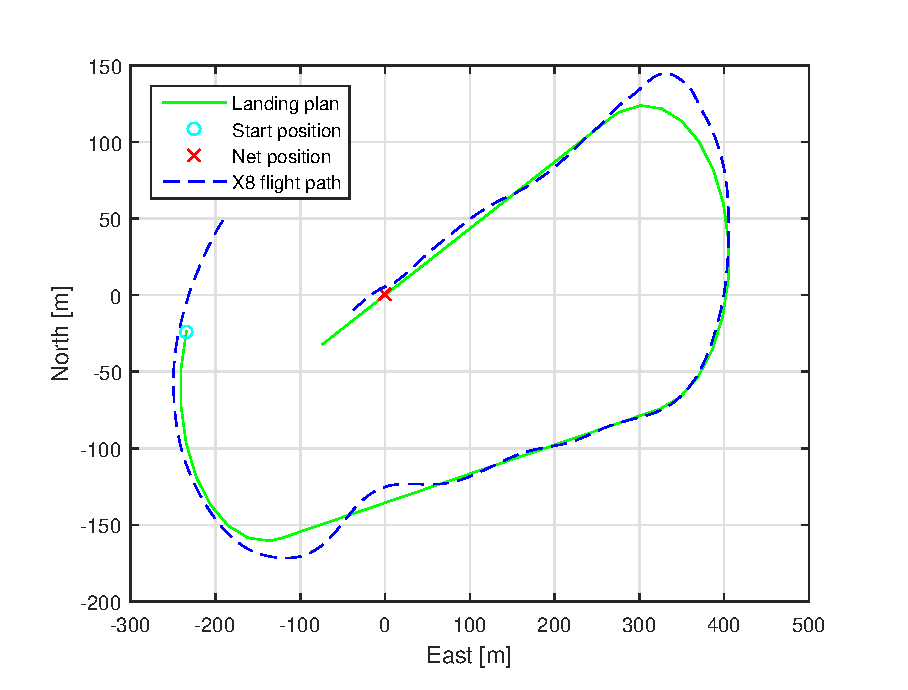
\includegraphics[scale=0.7]{figs/Experiment/NorthEast31mai125420.eps}
	\caption{North-East plot where the start and finish turning direction have the same turning direction}
	\label{Fig:NorthEast31mai125420}
\end{figure}

\subsection{Day 1}
\subsubsection{Path with reduced lookahead distance in lateral controller}
In order to further reduce the oscillatory motion in the lateral plan the lookahead distance in the lateral control system was reduced to make the controller more aggressive towards the wind. The effect of this change is shown in figure \ref{Fig:NorthEast31mai131844}, where the oscillatory motion is almost completely removed. However the reduced lookahead distance did not affect the the overshot in the finish turning circle.
\begin{figure}[H]
\centering
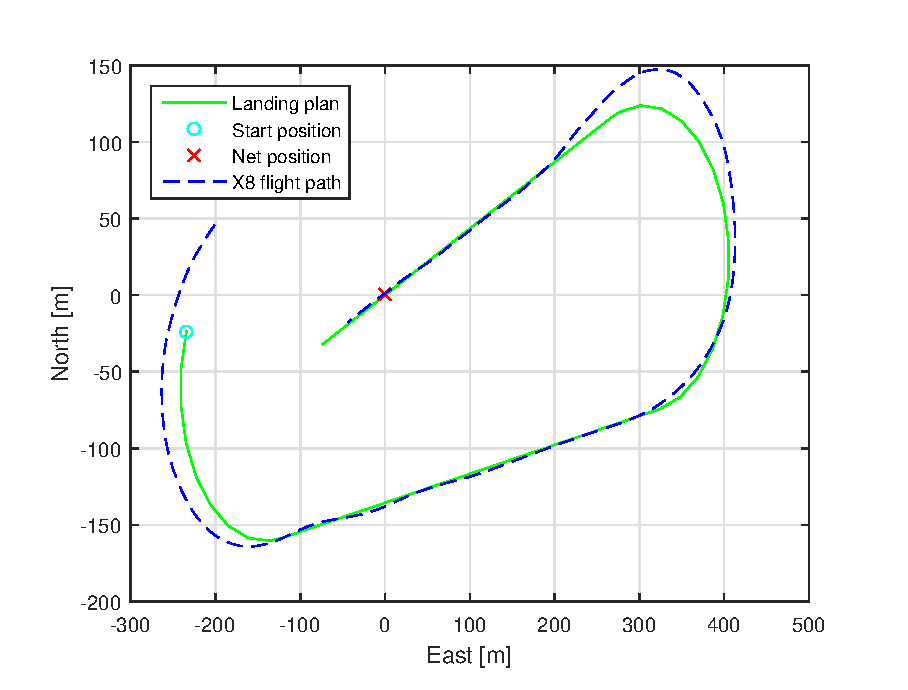
\includegraphics[scale=0.7]{figs/Experiment/NorthEast31mai131844.eps}
\caption{North-East plot where the lookahead distance of the lateral controller was reduced to increase performance of the autonomous landing system when flying against the wind}
\label{Fig:NorthEast31mai131844}
\end{figure}
By reviewing the desired roll ($\phi_d$ ) and the actual roll ($\phi$) of the \gls{uav} at the time of the final turn, shown in figure \ref{Fig:DesiredRoll131844}, it's observed that the lateral control system decrease the desired roll in the middle of the turn. This happens since the lateral control system only sees the next point on the circle, and not the circle as a whole.
\begin{figure}[H]
\centering
\includegraphics[scale=0.7]{figs/Experiment/rollDesired131844.eps}
\caption{The desired roll and actual roll of the \gls{uav} during the finish turning circle}
\label{Fig:DesiredRoll131844}
\end{figure}


%%%%%%
%\begin{table}[H]
%\centering
%\begin{tabular}{| l | l | l |}
%\hline
%\textbf{Nr.} 	& \textbf{Average height error [m]} 	& \textbf{Average cross track error [m]}  \\ \hline
%$1$				& $1.5$							& $6.1$								\\ \hline
%$2$				& $2.6$							& $6.7$								\\ \hline
%$3$				& $0.9$							& $5.5$								\\ \hline
%$4$				& $0.1$							& $2.8$								\\ \hline
%$5$				& $1.7$							& $2.0$								\\ \hline
%$6$				& $1.3$							& $6.8$								\\ \hline
%$7$				& $1,8$							& $9.1$								\\ \hline
%$8$				& $1.2$							& $8.2$								\\ \hline
%$9$				& $1.9$							& $5.9$								\\ \hline
%$10$			& $1.5$							& $4.4$								\\ \hline
%$11$			& $1.5$							& $1.4$								\\ \hline
%Average			& $1.5$							& $5.4$								\\ \hline
%Variance		& $0.4$							& $6.2$								\\ \hline
%\end{tabular}
%\caption{Mean height and cross track error from day 1}
%\label{tb:Day1HeightCrossTrack}
%\end{table}
%
%\begin{table}[H]
%
%\begin{tabular}{| p{0.5cm} | p{3cm} | p{4cm} | p{4cm} |}
%\hline
%\textbf{Nr.} & \textbf{Final approach angle [deg]} & \textbf{Lateral control system - Lookahead distance [m]} &  \textbf{Rotation combination - approach path}\\ \hline
%$1$				& $3$ &	$ 50 $ 	& Clockwise/Counter-clockwise		\\ \hline
%$2$				& $0$ & $ 50 $	& Clockwise/Counter-clockwise			\\ \hline
%$3$				& $0$ & $ 50 $	& Clockwise/Counter-clockwise		\\ \hline
%$4$				& $0$ & $ 50 $ 	& Counter-clockwise/ Counter-clockwise				\\ \hline
%$5$				& $0$ & $ 50 $ & Counter-clockwise/ Counter-clockwise					\\ \hline
%$6$				& $0$ & $ 50 $	& Counter-clockwise/ Counter-clockwise				\\ \hline
%$7$				& $0$ &	$ 50 $ & Counter-clockwise/ Counter-clockwise				\\ \hline
%$8$				& $0$ & $ 50 $	& Counter-clockwise/ Counter-clockwise				\\ \hline
%$9$				& $0$ & $ 50 $ & Counter-clockwise/ Counter-clockwise			\\ \hline
%$10$			& $0$ &	$ 30 $ & Counter-clockwise/ Counter-clockwise	\\ \hline
%$11$			& $0$ & $ 30 $ & Counter-clockwise/ Counter-clockwise\\ \hline
%\end{tabular}
%\caption{Table containing the result of each landing attempt}
%\label{tb:Day1LandingAttempt}
%\end{table}
%
%\begin{table}[H]
%\centering
%\begin{tabular}{| p{0.5cm} | p{1cm} | p{1cm} | p{3.5cm} | p{3cm} | p{1cm} |}
%\hline
%\textbf{Nr.}	& \textbf{Height error [m]}	& \textbf{Cross track error [m]}& \textbf{Height acceptance}& \textbf{Cross track error acceptance}	& \textbf{Net hit}\\ \hline
%$1$				& $2.8$		& $2.1$		& X								& OK									& X					\\ \hline
%$2$				& $2.7$		& $-4.5$	& X								& X										& X					\\ \hline
%$3$				& $0.9$		& $-1.6$	& OK							& OK									& OK				\\ \hline
%$4$				& $0.0$		& $5.4$		& OK							& X										& X					\\ \hline
%$5$				& $0.8$		& $5.3$		& OK							& X										& X					\\ \hline
%$6$				& $2.1$		& $-1.6$	& X								& OK									& X					\\ \hline
%$7$				& $0.7$		& $2.3$		& OK							& OK									& OK				\\ \hline
%$8$				& $-1.5$	& $-5.4$	& X								& X										& X					\\ \hline
%$9$				& $1.9$		& $0.8$		& X								& OK									& X					\\ \hline
%$10$			& $0.3$	& $1.1$		& OK							& OK									& OK				\\ \hline
%$11$			& $-1.3$	& $0.2$		& OK							& OK									& OK				\\ \hline
%\end{tabular}
%\caption{Table containing the result of each landing attempt}
%\label{tb:Day1LandingAttempt}
%\end{table}
%%%%%%
%\begin{table}
%\centering
%\begin{tabular}{| l | l | l | l |}
%\hline
%\textbf{Nr.}	&  \textbf{Height acceptance}& \textbf{Cross track error acceptance}	& \textbf{Net hit}\\ \hline
%$1$				& X								& OK									& X					\\ \hline
%$2$				& X								& X										& X					\\ \hline
%$3$				& OK							& OK									& OK				\\ \hline
%$4$				& OK							& X										& X					\\ \hline
%$5$				& OK							& X										& X					\\ \hline
%$6$				& X								& OK									& X					\\ \hline
%$7$				& OK							& OK									& OK				\\ \hline
%$8$				& X								& X										& X					\\ \hline
%$9$				& X								& OK									& X					\\ \hline
%$10$			& OK							& OK									& OK				\\ \hline
%$11$			& OK							& OK									& OK				\\ \hline
%\end{tabular}
%\end{table}




The longitudinal control system showed a stable performance, however a large average error in the height with respect to the desired height shows a performance that is not acceptable for a autonomous landing system. Compared to the results obtain in the SIL simulation \ref{SIL:Results} where the low level controllers are fined tuned, shows that the performance can be increased by further tuning of the low level pitch controller. This might allow for an increased glide slope angle, which will increase the height difference between the landing net and the start of the landing path or reduce the necessary glide slope length. However the risk with an increased glide slope angle is an increased airspeed, which could result in a large overshot with respect to the desired height. 

The lateral control system performed with satisfying result during the second day when the wind condition was calm, however during the first day it experienced problems when attempting to converge to the straight line between two waypoints. This result differ from the SIL simulation of the autonomous landing system, which was expected due to the mathematical model used to represent the X8 \gls{uav} has not been verified against a physical model of the X8, in addition to the low level controllers not being fined tuned for autonomous flights. The lateral control system  struggeled to avoid overshooting when following the finish turning circle, with some resulting overshot large enough to bring the \gls{uav} to the edged of the operational flight space. During the flight experiments some key factors was identified which resulted in increased performance from the lateral control system. The key factors are listed in table \ref{Tb:KeyAlterationFactorsLateral}.
\begin{table}[H]
\begin{itemize}
\item Reducing the lookahead distance when flying in strong wind conditions.
\item Creation of a approach path with the same rotation direction in both turning circles.
\item Reducing the distance between each arc segments in the turning circles.
\end{itemize}
\caption{Alteration in the autonomous landing system which resulted in increased performance from the lateral controller}
\label{Tb:KeyAlterationFactorsLateral}
\end{table}
The reduction of the lookahead distance will result in increased performance when against the wind, at the cost of reduced performance when flying in the tail wind. A possible solution to this problem would be to implement the the lookahead distance as a function of the cross track error, which in \citep{fossen2011handbook} section 10.3.2 is given as:
\begin{equation}
\Delta(t) = \sqrt{R^2 - e(t)^2}
\end{equation}
where $\Delta(t)$ is the lookahead distance, $R$ is the maximum lookahead distance and $e(t)$ is the cross track error. In addition the lateral control system functionality could be expanded to increase the performance during a turning manoeuvre, with the goal of reducing the overshot.

Experimentation with the landing plan parameter showed that both the lateral and longitudinal control system was affected by the choice of parameters. During the first day the rotation direction of the start turning circle brought the \gls{uav} into the cross wind, which caused oscillatory motion in the \gls{uav}. Thus the combination of rotation direction should be considered carefully, with the recommended combination being either counter-clockwise/counter-clockwise or clockwise/clockwise. These combinations will result a smoother transition between the two turning circles, hence reduce the oscillation in the lateral controller. In addition the final approach angle must be zero, in order for the longitudinal control system to output a desire height reference which equals the net center height. Other key landing plan factors with recommended values for increase autonomous landing system performance are listed in table \ref{Tb:RecommmendedLandingPlanParameter}.
\begin{table}[H]
\centering
\begin{tabular}{| l | l |}
\hline
\textbf{Parameter name}			&  \textbf{Recommended value} 	\\ \hline
Time of arrival factor			&	$2 s$						\\ \hline
Distance between arc segments	&	$10 m$					 	\\ \hline
Final approach length			&	$100 m$					 	\\ \hline
Final approach angle			&   $0 \deg$					\\ \hline
Glide slope angle				&	$6 \deg$				 	\\ \hline
\end{tabular}
\caption{Recommended parameter alteration to the landing plan with respect to the plan parameter given in table \ref{AP:TB:landingDay2}, and the task configuration parameter given in table \ref{Tb:LandingPlanParameter}}
\label{Tb:RecommmendedLandingPlanParameter}
\end{table}
The minimum height from which the autonomous landing system could start the landing path from was found to be $56 m$ above the runway at Agdenes airfield when attempting to land from the east. This strain the operation boundaries in which the \gls{uav} operates, since the approach could move the \gls{uav} out of the line of sight of the pilot. An alternative approach from the west is possible, however the typical wind condition on Agdenes is from the west, which would limit the weather window of the autonomous landing system.
